\section{问题四：波动电价下的扩展}
\subsection{价格预测与问题4-2}
未来实际价格不可见，故对电价同样采用式~\eqref{eq:forecast}的历史滚动预测，实际价格只用于事后结算。价格预测MAE和WAPE分别为0.0532元/kWh和6.94\%，预测与实际日均价格见图~\ref{fig:price}。
\begin{figure}[H]\centering
\includegraphics[width=0.90\textwidth]{../figures/fig06_price_forecast.pdf}
\caption{波动电价的历史滚动预测与实际值}\label{fig:price}\end{figure}
问题4-2将预测价格代入问题二的目标函数，按实际价格事后结算的累计费用为16,108,523.19元。该口径把预测价格用于决策、真实价格仅用于评价，避免把事后价格曲线泄漏进日前计划。
\subsection{问题4-3与综合比较}
问题4-3同时在发布时点更新光伏预测，并根据已观察价格偏差修正剩余时段价格预测。8种组合中不调整以16,569,050.38元最低；最佳非空组合为仅6:00更新，费用17,138,646.42元。图~\ref{fig:compare}同时给出固定价与波动价下的组合排序，表明高调整罚金下全时点更新并非必然最优。
\begin{figure}[H]\centering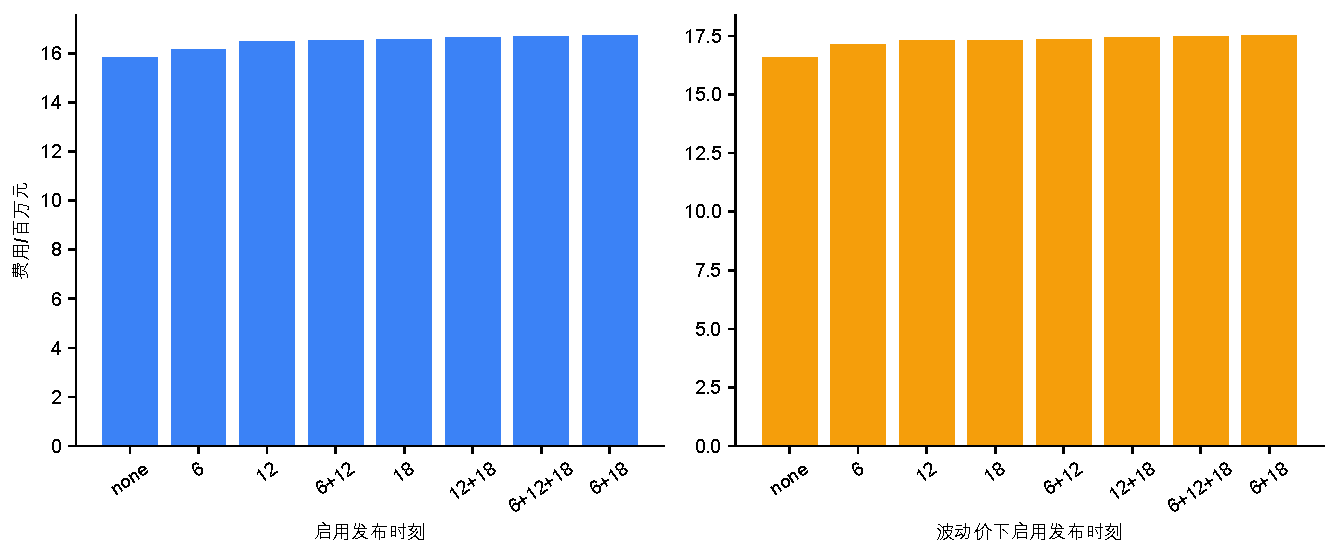
\includegraphics[width=0.92\textwidth]{../figures/fig03_combo_comparison.pdf}
\caption{固定价与波动价下8种更新组合累计费用}\label{fig:compare}\end{figure}
\begin{table}[H]\centering\caption{四个指定日期的主模型总费用（元）}\label{tab:selected}\small
\begin{tabular}{lrrrr}\toprule 日期 & 问题二 & 问题三 & 问题4-2 & 问题4-3\\\midrule
2025-03-20 & 44,643.13 & 58,465.72 & 45,189.83 & 59,961.07\\
2025-06-21 & 31,552.20 & 30,583.44 & 29,674.44 & 26,238.07\\
2025-09-23 & 56,659.21 & 50,441.33 & 58,452.46 & 52,794.43\\
2025-12-21 & 66,252.63 & 66,821.64 & 77,718.02 & 78,830.69\\\bottomrule
\end{tabular}\end{table}
